\newpage
\section{Ôn tập chương 9}
\def\thoigian{90}%--Thời gian
\de{Đề số 1}{Chương IX. Phương pháp tọa độ trong mặt phẳng}


\begin{center}
	\textbf{PHẦN 1 - CÂU TRẮC NGHIỆM BỐN PHƯƠNG ÁN}
\end{center}
\Opensolutionfile{ans}[ans/ans-TN-ONTAPCHUONGIX-DE1]

\begin{ex}%[0H9N1-3]%[Dự án D - đợt 2 NH24-25- Quang Vinh NT]
	Trong mặt phẳng tọa độ $Oxy$, cho hai điểm $A(1;4)$ và $B(3;5)$. Khi đó
	\choice
	{$\overrightarrow{AB}=(4;9)$}
	{$\overrightarrow{AB}=(1;2)$}
	{\True $\overrightarrow{AB}=(2;1)$}
	{$\overrightarrow{AB}=(-2;-1)$}
	\loigiai{
		$\overrightarrow{AB}=(3-1;5-4)=(2;1)$.
	}
\end{ex}
\begin{ex}%[0H9N1-1]%[Dự án D - đợt 2 NH24-25- Quang Vinh NT]
	Trong mặt phẳng tọa độ $Oxy$, tọa độ của $\overrightarrow{u}=-3\overrightarrow{i}+5\overrightarrow{j}$ là
	\choice
	{\True $\overrightarrow{u}=(-3; 5)$}
	{$\overrightarrow{u}=(3;-5)$}
	{$\overrightarrow{u}=(-5; 3)$}
	{$\overrightarrow{u}=(5;-3)$}
	\loigiai{
		Ta có $\overrightarrow{u}=-3\overrightarrow{i}+5\overrightarrow{j} \Leftrightarrow \overrightarrow{u}=(-3; 5)$.
	}
\end{ex}
\begin{ex}%[0H9H1-2]%[Dự án đề kiểm tra HKII NH22-23- Mui Doan]%[THPT Nguyễn Thái Bình]
	Trong mặt phẳng tọa độ $Oxy$, cho $\overrightarrow{a}=(-1 ; 2)$, $ \overrightarrow{b}=(5 ;-7)$. Tọa độ của véc-tơ $\overrightarrow{a}-\overrightarrow{b}$ là
	\choice
	{\True $(-6 ; 9)$}
	{$(-5 ;-14)$}
	{$(6 ;-9)$}
	{$(4 ;-5)$}
	\loigiai
	{
		Ta có $\overrightarrow{a}-\overrightarrow{b}=(-6 ; 9)$.
	}
\end{ex}

\begin{ex}%[0H9N3-1]%[Dự án D - đợt 2 NH24-25- Quang Vinh NT]
	Trong mặt phẳng tọa độ $Oxy$, cho đường thẳng $d\colon \dfrac{x}{3} + \dfrac{y}{5} = 1$. Một véc-tơ pháp tuyến của $d$ là
	\choice
	{$\overrightarrow{n}_1 = (3;5)$}
	{$\overrightarrow{n}_2 = (3;-5)$}
	{$\overrightarrow{n}_3 = (-5;3)$}
	{\True$\overrightarrow{n}_4 = (5;3)$}
	\loigiai{
		đường thẳng $d\colon \dfrac{x}{3} + \dfrac{y}{5} = 1\Leftrightarrow 5x +3y-15=0$ có một véc-tơ pháp tuyến là $\overrightarrow{n}_4 = (5;3)$.
	}
\end{ex}
\begin{ex}%[0H9H3-2]%[Dự án D - đợt 2 NH24-25- Quang Vinh NT]
	Trong mặt phẳng tọa độ $Oxy$, phương trình tham số của đường thẳng $d$ đi qua điểm $M(4;-5)$ và có một véc-tơ chỉ phương là $\overrightarrow{u}=(1;0)$ là
	\choice
	{\True $\heva{&x=4+t\\&y=-5}$}
	{$\heva{&x=1+4t\\&y=-5t}$}
	{$\heva{&x=4\\&y=-5+t}$}
	{$\heva{&x=4\\&y=-5}$}
	\loigiai{
		$d$ đi qua điểm $M(4;-5)$ và có một véc-tơ chỉ phương là $\overrightarrow{u}=(1;0)$ nên có phương trình $\heva{&x=4+t\\&y=-5.}$
	}
\end{ex}
\begin{ex}%[0H9H3-3]%[Dự án D - đợt 2 NH24-25- Quang Vinh NT]
	Trong mặt phẳng tọa độ $Oxy$, xác định vị trí tương đối của hai đường thẳng có phương trình sau: $d_1\colon 2x-y+1=0$ và $d_2\colon -4x+2y+2=0$.
	\choice
	{Cắt nhau}
	{Vuông góc nhau}
	{Trùng nhau}
	{\True Song song nhau}
	\loigiai{
		Ta có: $\dfrac{2}{-4}=\dfrac{-1}{2}\ne\dfrac{1}{2}$ suy ra $d_1$ song song với $d_2$.
	}
\end{ex}
\begin{ex}%[0H9N4-1]%[Dự án D - đợt 2 NH24-25- Quang Vinh NT]
	Trong mặt phẳng tọa độ $Oxy$,  đường tròn $(C)\colon x^2 + y^2 - 2x + 6y + 1 = 0$ có tâm $I$ và bán kính $R$ là
	\choice
	{$I(2;-6)$ và $R=\sqrt{39}$}
	{$I(1;-3)$ và $R=\sqrt{10}$}
	{\True $I(1;-3)$ và $R=3$}
	{$I(-1;3)$ và $R=3$}
	\loigiai{
		Ta có $x^2 + y^2 - 2x + 6y + 1 = 0\Leftrightarrow (x-1)^2 + (y+3)^2 = 9$.\\
		Đường tròn đã cho có tâm $I(1;-3)$ và bán kính $R=\sqrt{9}=3$.
	}
\end{ex}
\begin{ex}%[0H9H4-2]%[Dự án D - đợt 2 NH24-25- Quang Vinh NT]
	Trong mặt phẳng tọa độ $Oxy$, phương trình đường tròn tâm $I(-3;4)$, có bán kính $R=2$ là
	\choice
	{$(x-3)^2 + (y-4)^2 = 4$}
	{\True $(x+3)^2 + (y-4)^2 =4$}
	{$(x+3)^2 + (y+4)^2 = 4$}
	{$(x+3)^2 + (y-4)^2 = 2$}
	\loigiai{
		Phương trình đường tròn tâm $I(-3;4)$, có bán kính $R=2$ là
		\begin{equation*}
			(x+3)^2 + (y-4)^2 = 4.
		\end{equation*}
	}
\end{ex}
\begin{ex}%[0H9H4-3]%[Dự án D - đợt 2 NH24-25- Quang Vinh NT]
	Trong mặt phẳng tọa độ $Oxy$, phương trình tiếp tuyến của đường tròn $(C)\colon (x+1)^2+(y-2)^2=29$ tại điểm $M(-3;7)$ là
	\choice
	{$2x+5y-41=0$}
	{$4x-5y+47=0$}
	{\True $2x-5y+41=0$}
	{$2x-5y-29=0$}
	\loigiai{
		Đường tròn $(C)$ có tâm $I(-1;2)$.\\
		Tiếp tuyến của $(C)$ tại $M(-3;7)$ đi qua $M(-3;7)$ và nhận $\overrightarrow{IM} = (-2;5)$ làm một véc-tơ pháp tuyến, có phương trình $$-2(x+3) + 5(y-7) = 0\Leftrightarrow -2x+5y-41=0\Leftrightarrow 2x-5y+41=0.$$
	}
\end{ex}

\begin{ex}%[0H9H5-2]%[Dự án D - đợt 2 NH24-25- Quang Vinh NT]
	Trong mặt phẳng tọa độ $Oxy$,  cho elip có phương trình $9{x^2}+25{y^2}=225$. Tiêu cự của elip bằng
	\choice
	{$6$}
	{$15$}
	{\True $8$}
	{$4$}
	\loigiai{
		Phương trình elip $(E)$ có dạng $9{x^2}+25{y^2}=225\Leftrightarrow \dfrac{{x^2}}{25}+\dfrac{{y^2}}{9}=1$.\\
		Theo bài ra ta có $\heva{& {a^2}=25 \\ & {b^2}=9 .}$\\
		Mà $ c=\sqrt {{a^2}-{b^2}}=\sqrt {25-9}=\sqrt {16}=4$.\\
		Vậy tiêu cự của elip đã cho là $2c=8$.}
\end{ex}
\begin{ex}%[0H9H5-5]%[Dự án D - đợt 2 NH24-25- Quang Vinh NT]
	Trong mặt phẳng tọa độ $Oxy$, hypebol cắt trục hoành tại điểm $A( 4;0 )$ và một tiêu điểm $F_1( -5;0 )$ có phương trình chính tắc là
	\choice
	{\True $\dfrac{{x^2}}{16}-\dfrac{{y^2}}{9}=1$}
	{$\dfrac{{y^2}}{16}+\dfrac{{x^2}}{9}=1$}
	{$\dfrac{{y^2}}{16}-\dfrac{{x^2}}{9}=1$}
	{$\dfrac{{x^2}}{16}-\dfrac{{y^2}}{25}=1$}
	\loigiai{
		Phương trình chính tắc của hypebol có dạng $\dfrac{{x^2}}{{a^2}}-\dfrac{{y^2}}{{b^2}}=1\,\,(a,b>0)$.\\
		Ta có : $\heva{& \dfrac{16}{{a^2}}=1 \\ & c=5 \\ & {b^2}={c^2}-{a^2} }$ $\Rightarrow \heva{& {a^2}=16 \\ & {c^2}=25 \\ & {b^2}=9 .} $\\
		Phương trình chính tắc của hypebol là $\dfrac{{x^2}}{16}-\dfrac{{y^2}}{9}=1.$}
\end{ex}

\begin{ex}%[0H9H5-7]%[Dự án D - đợt 2 NH24-25- Quang Vinh NT]
	Tiêu điểm của parabol $y^2=\sqrt {3}x$ là
	\choice
	{$F\left( -\dfrac{\sqrt {3}}{4};0 \right)$}
	{$F\left( \dfrac{\sqrt {3}}{2};0 \right)$}
	{$F\left( -\dfrac{\sqrt {3}}{2};0 \right)$}
	{\True $F\left( \dfrac{\sqrt {3}}{4};0 \right)$}
	\loigiai{
		Ta có $ p=\dfrac{\sqrt {3}}{2}$ $\Rightarrow F\left( \dfrac{\sqrt {3}}{4};0 \right)$. }
\end{ex}

\Closesolutionfile{ans}
%\begin{center}
%	\textbf{ĐÁP ÁN}
%	\inputansbox{10}{ans/ans}	
%\end{center}

\begin{center}
	\textbf{PHẦN 2 - CÂU TRẮC NGHIỆM ĐÚNG SAI}
\end{center}

\Opensolutionfile{ans}[ans/answer-DS-ONTAPCHUONGIX-DE1]

\begin{ex}%[0H9V3-5]%[Dự án D - đợt 2 NH24-25- Quang Vinh NT]
	Trong mặt phẳng toạ độ $Oxy$, cho tam giác $ABC$ có $A(1;1)$, $B(2;4)$, $C(5;1)$.
	\choiceTF
	{Đường cao $AH$ có phương trình $x-y+1=0$}
	{\True Đường trung tuyến $CE$ có một véc-tơ chỉ phương là $\overrightarrow{u}=(7;-3)$}
	{$\cos (AH,CE)=\dfrac{1}{\sqrt{29}}$}
	{\True Các đường thẳng đi qua $B$ và cách đều $2$ điểm $A$ và $C$ có phương trình lần lượt là $y-4=0$ và $ax+by-10=0$. Khi đó $a+b=4$}
	\loigiai{
		\begin{itemchoice}
			\itemch Đường cao $AH$ có véc-tơ pháp tuyến là $\overrightarrow{BC}=(3;-3)$.\\
			Khi đó $AH\colon 3(x-1)-3(y-1)=0$ hay $AH\colon x-y=0$.
			\itemch Tọa độ trung điểm $E$ của $AB$ là $\left( \dfrac{3}{2};\dfrac{5}{2}\right) $.\\
			Ta có $\overrightarrow{CE}=\left(-\dfrac{7}{2};\dfrac{3}{2}\right) =-\dfrac{1}{2}(7;-3)$.\\
			Suy ra đường trung tuyến $CE$ có một véc-tơ chỉ phương là $\overrightarrow{u}=(7;-3)$.
			\itemch 
			\begin{itemize}
				\item $AH$ có véc-tơ chỉ phương là $\overrightarrow{a}=(1;1)$.
				\item $CE$ có véc-tơ chỉ phương là $\overrightarrow{u}=(7;-3)$.
				\item $\cos (AH,CE)=\dfrac{\left|\overrightarrow{a}\cdot \overrightarrow{u}\right|}{\left|\overrightarrow{a}\right|\cdot\left|\overrightarrow{u}\right|}=\dfrac{\left| 1\cdot 7+1\cdot(-3)\right|}{\sqrt{1^2+1^2}\cdot \sqrt{7^2+(-3)^2}}=\dfrac{4}{2\sqrt{29}}=\dfrac{2}{\sqrt{29}}$.
			\end{itemize}
			\itemch Gọi $\Delta$ là đường thẳng đi qua điểm $B(2;4)$. Khi đó $\Delta\colon ax+by-2a-4b=0$.\\
			Ta có 
			\allowdisplaybreaks
			\begin{eqnarray*}
				\mathrm{d}(A,\Delta)=\mathrm{d}(C,\Delta)&\Leftrightarrow&\dfrac{\left|-a-3b\right| }{\sqrt{a^2+b^2}}=\dfrac{\left|3a-3b\right| }{\sqrt{a^2+b^2}}\\
				&\Leftrightarrow& \left|-a-3b\right|=\left|3a-3b\right|\\
				&\Leftrightarrow& \hoac{&-a-3b=3a-3b\\&-a-3b=-3a+3b}\\
				&\Leftrightarrow& \hoac{&a=0\\&a=3b}\\
				&\Leftrightarrow& \hoac{&\heva{&a=0\\&b=1}\\&\heva{&a=3\\&b=1.}}
			\end{eqnarray*}
			Suy ra $\Delta\colon y-4=0$ hay $\Delta\colon 3x+y-10=0$.\\
			Do đó $a+b=3+1=4$.
	\end{itemchoice}}
\end{ex}

\begin{ex}%[0H9V4-5]%[Dự án D - đợt 2 NH24-25- Quang Vinh NT]
	Trong mặt phẳng tọa độ $Oxy$, cho đường tròn $(C)\colon (x-1)^2+(y-2)^2=25$ và đường thẳng $d\colon 4x-3y+3=0$.
	\choiceTF
	{Đường thẳng $d$ có một véc-tơ pháp tuyến là $\overrightarrow{n}=(3;4)$}
	{\True Đường tròn $(C)$ có tâm $I(1;2)$, bán kính $R=5$}
	{\True Đường thẳng có phương trình $3x+4y+14=0$ là một tiếp tuyến của đường tròn $(C)$ và vuông góc với đường thẳng $d$}
	{\True Phương trình của đường tròn $(C')$ tâm $I'(1;-1)$ tiếp xúc với đường thẳng $d$ là $(x-1)^2+(y+1)^2=4$}
	\loigiai{
		\begin{itemchoice}
			\itemch Đường thẳng $d$ có $1$ véc-tơ chỉ phương là $\overrightarrow{u}=(3;4)$.
			\itemch Đường tròn $(C)$ có tâm $I(1;2)$, bán kính $R=5$.
			\itemch 
			\begin{itemize}
				\item \textbf{Cách 1:} Nhận thấy đường thẳng $\Delta$ có phương trình $\Delta \colon 3x+4y+14=0$ vuông góc với đường thẳng $d$.\\
				Lại có $\mathrm{d}(I,\Delta)=\dfrac{|3\cdot1+4\cdot2+14|}{\sqrt{3^2+4^2}}=5=R$ nên $\Delta$ là một tiếp tuyến của $(C)$.
				\item \textbf{Cách 2:} Gọi $\Delta$ là tiếp tuyến của $(C)$ và vuông góc với $d$. Khi đó $\Delta \colon 3x+4y+c=0$.\\
				Vì $\Delta$ là tiếp tuyến của $(C)$ nên $\mathrm{d}(I,\Delta)=R\Rightarrow\dfrac{|3\cdot1+4\cdot2+c|}{\sqrt{3^2+4^2}}=5\Rightarrow\hoac{&c=14\\&c=-36.}$\\
				Vậy $\Delta \colon 3x+4y+14=0$ hoặc $\Delta\colon 3x+4y-36=0$.
			\end{itemize}
			\itemch 
			Vì $(C')$ có tâm $I'(1;-1)$ tiếp xúc với đường thẳng $d$ nên $(C')$ có bán kính là \begin{eqnarray*}
				R'=\mathrm{d}(I',d)=\dfrac{|4\cdot1-3\cdot(-1)+3|}{\sqrt{4^2+(-3)^2}}=2.
			\end{eqnarray*}
			Phương trình của đường tròn $(C')$ tâm $I'(1;-1)$, bán kính $R'=2$ là \begin{eqnarray*}
				(x-1)^2+(y+1)^2=4.
			\end{eqnarray*}
		\end{itemchoice}
	}
\end{ex}
\Closesolutionfile{ans}
%\inputansbox[2]{2}{ans/answer.tex}

\begin{center}
	\textbf{PHẦN 3 - CÂU TRẮC NGHIỆM TRẢ LỜI NGẮN}
\end{center}
\setcounter{ex}{0}
\Opensolutionfile{ans}[ans-KQ-ONTAPCHUONGIX-DE1]

\begin{ex}%[0H9H3-5]%[Dự án D - đợt 2 NH24-25- Quang Vinh NT]
	Trong mặt phẳng $xOy$ cho điểm $S(x;y)$ di động trên đường thẳng $d$ có phương trình $3x-$ $4y+7=0$. Tính khoảng cách ngắn nhất từ điểm $A(1;3)$ đến điểm $S(x; y)$. (làm tròn đến hàng phần chục)
	
	\shortans{0,4}
	\loigiai{
		Khoảng cách ngắn nhất từ điểm $A(1;3)$ đến điểm $S(x; y)$ là $$\mathrm{d}(A,d)=\dfrac{|3\cdot 1-4\cdot 3+7|}{\sqrt{3^2+(-4)^2}}=\dfrac{2}{5}=0{,}4.$$
	}
\end{ex}

\begin{ex}%[0H9V4-2]%[Dự án D - đợt 2 NH24-25- Quang Vinh NT]
	Trong mặt phẳng $Oxy$, biết bán kính đường tròn đi qua ba điểm $A(3;0)$, $B(1;6)$ và $C(-5;0)$ là $R$. Tính $R^2$.
	
	\shortans{20}
	\loigiai{
		Gọi $I(x;y)$ là tâm đường tròn ngoại tiếp tam giác $ABC$.\\
		Ta có\\
		$IA^2=(x-3)^2+y^2=x^2 -6x+9+y^2$; \\
		$IB^2=(x-1)^2+(y-6)^2=x^2 -2x+y^2 -12y+37$; \\
		$IC^2=(x+5)^2+y^2=x^2 +10x+25+y^2$.\\
		Suy ra
		\begin{eqnarray*}
			&&\heva{&IA^2=IB^2\\&IA^2=IC^2}\\
			&\Leftrightarrow &\heva{&x^2 -6x+9+y^2=x^2 -2x+y^2 -12y+37\\&x^2 -6x+9+y^2=x^2 +10x+25+y^2}\\
			&\Leftrightarrow& \heva{&-6x+9=-2x -12y+37 \\ &-6x+9=10x+25} \\
			&\Leftrightarrow&\heva{&-4x+12y=28 \\ &-16x=16}\\ &\Leftrightarrow& \heva{&x=-1 \\ &y=2.}
		\end{eqnarray*}
		Tâm đường tròn là $I(-1;2)$.\\
		Vậy $R^2=IA^2=(-1-3)^2+2^2=20$.
	}
\end{ex}

\begin{ex}%[0H9V4-7]%[Dự án D - đợt 2 NH24-25- Quang Vinh NT]
	Bác Bình có một cái ao cá, giữa ao là một khu đất hình tròn bán kính $1{,}5$\,m  (xem hình vẽ). Bác Bình muốn xây một cây cầu nối từ phần đất liền (là tam giác $ABC$) nối ra khu đất. Biết $AC = 5$\,m, $AB = 2$\,m và $IH = 2$\,m, $IK = 5$\,m. Chiều dài cây cầu ngắn nhất mà Bác Bình có thể xây là bao nhiêu mét (làm tròn kết quả đến hàng phần mười)?
	\begin{center}
		\begin{tikzpicture}[scale=0.8, font=\footnotesize, line join=round, line cap=round,>=stealth]
			% Dat cac diem dua tren he truc toa do
			\path
			(0,0) coordinate (C)
			(0,5) coordinate (A)
			(2,5) coordinate (B)
			(5,2) coordinate (I)
			(0,2) coordinate (K) % Hinh chieu cua I len AC
			(5,0) coordinate (H) % Hinh chieu cua I len truc hoanh
			(7,5) coordinate (M) % Diem phu de ve hinh chu nhat bao ngoai
			(7,0) coordinate (N);
			% Ve hinh chu nhat bao ngoai
			\draw (A)--(M)--(N)--(C)--(A);
			% Ve va to mau khu dat lien (hinh thang vuong AC'BA voi C' la (2,0))
			\fill[pattern=north east lines, pattern color=blue] (A)--(B)--(C)--cycle;
			\draw (A)--(B)--(C); % Ve cac canh cua khu dat
			% Ve va to mau khu dat tron
			\fill[blue, opacity=0.3] (I) circle (1.5cm);
			\draw[blue] (I) circle (1.5cm);
			% Ve cac duong giong net dut
			\draw[dashed] (I)--(K);
			\draw[dashed] (I)--(H);
			% Ve va dat ten cac diem
			\foreach \p/\q in {A/135, B/90, C/-135, I/0, K/180, H/-90,M/90,N/-90}
			\fill[black] (\p) circle (1.5pt) node[shift={(\q:3.5mm)}]{$\p$};
			\draw pic[draw=black,angle radius=0.2cm] {right angle = B--A--C};
			\draw pic[draw=black,angle radius=0.2cm] {right angle = K--C--H};
			\draw pic[draw=black,angle radius=0.2cm] {right angle = I--K--C};
			\draw pic[draw=black,angle radius=0.2cm] {right angle = I--H--C}; 
		\end{tikzpicture}
	\end{center}
	\shortans{2,4}
	\loigiai{
		Để giải bài toán, ta thiết lập một hệ trục toạ độ $Oxy$ sao cho điểm $C$ trùng với gốc toạ độ $O(0;0)$, trục $Oy$ chứa đoạn thẳng $AC$ và trục $Ox$ đi qua điểm $H$.
		\begin{center}
			\begin{tikzpicture}[scale=0.8, font=\footnotesize, line join=round, line cap=round,>=stealth]
				% Dat cac diem dua tren he truc toa do
				\path
				(0,0) coordinate (C)
				(0,5) coordinate (A)
				(2,5) coordinate (B)
				(5,2) coordinate (I)
				(0,2) coordinate (K) % Hinh chieu cua I len AC
				(5,0) coordinate (H) % Hinh chieu cua I len truc hoanh
				(7,5) coordinate (M) % Diem phu de ve hinh chu nhat bao ngoai
				(7,0) coordinate (N)
				($(C)!1.2!(N)$)coordinate (x)
				($(C)!1.2!(A)$)coordinate (y)
				($(C)!-0.3!(H)$)coordinate (x')
				($(C)!-0.2!(K)$)coordinate (y')
				;
				% Ve hinh chu nhat bao ngoai
				\draw (A)--(M)--(N)--(C)--(A);
				% Ve va to mau khu dat lien (hinh thang vuong AC'BA voi C' la (2,0))
				\fill[pattern=north east lines, pattern color=blue] (A)--(B)--(C)--cycle;
				\draw (A)--(B)--(C); % Ve cac canh cua khu dat
				% Ve va to mau khu dat tron
				\fill[blue, opacity=0.3] (I) circle (1.5cm);
				\draw[blue] (I) circle (1.5cm);
				% Ve cac duong giong net dut
				\draw[dashed] (I)--(K);
				\draw[dashed] (I)--(H);
				% Ve va dat ten cac diem
				\foreach \p/\q in {A/135, B/90, C/-135, I/0, K/180, H/-90,M/90,N/-90}
				\fill[black] (\p) circle (1.5pt) node[shift={(\q:3.5mm)}]{$\p$};
				\draw pic[draw=black,angle radius=0.2cm] {right angle = B--A--C};
				\draw pic[draw=black,angle radius=0.2cm] {right angle = K--C--H};
				\draw pic[draw=black,angle radius=0.2cm] {right angle = I--K--C};
				\draw pic[draw=black,angle radius=0.2cm] {right angle = I--H--C}; 
				\draw[->](x')--(x) node[below]{$x$};
				\draw[->](y')--(y) node[right]{$y$};
			\end{tikzpicture}
		\end{center}
		\begin{itemize}
			\item Do $C(0;0)$ và $AC=5\,\mathrm{m}$, ta có toạ độ điểm $A$ là $A(0;5)$.
			\item Do $AB=2\,\mathrm{m}$ và $AB$ song song với trục $Ox$, ta có toạ độ điểm $B$ là $B(2;5)$.
			\item Từ hình vẽ, ta có toạ độ tâm $I$ của khu đất hình tròn là $I(5;2)$.
			\item Bán kính của khu đất là $R=1{,}5$\,m.
		\end{itemize}
		Cây cầu là đoạn thẳng ngắn nhất nối một điểm trên đoạn $BC$ với một điểm trên đường tròn tâm $I$.
		\\
		Phương trình đường thẳng chứa đoạn $BC$ đi qua $C(0;0)$ và $B(2;5)$ có dạng $y=\dfrac{5}{2}x$ hay $5x-2y=0$.
		\\
		Khoảng cách từ tâm $I$ đến đường thẳng $BC$ là
		$$\mathrm{d}(I,BC)=\dfrac{|5 \cdot 5 - 2 \cdot 2|}{\sqrt{5^2+(-2)^2}} = \dfrac{21}{\sqrt{29}}.$$
		Gọi $M$ là hình chiếu của $I$ trên đường thẳng $BC$. Toạ độ điểm $M$ là nghiệm của hệ phương trình
		$$\heva{&5x-2y=0\\&2(x-5)+5(y-2)=0} \Leftrightarrow \heva{&x=\dfrac{40}{29}\\&y=\dfrac{100}{29}}$$
		Vì $0 < x_M = \dfrac{40}{29} < 2$ nên điểm $M$ thuộc đoạn thẳng $BC$.
		\\
		Do đó, chiều dài cây cầu ngắn nhất bằng khoảng cách từ $I$ đến đường thẳng $BC$ trừ đi bán kính $R$.
		\\
		Chiều dài cây cầu là $l= \mathrm{d}(I,BC)-R = \dfrac{21}{\sqrt{29}} - 1{,}5 \approx 2{,}3996\,(\mathrm{m})$.
		\\
		Làm tròn kết quả đến hàng phần mười, ta được $2{,}4\,\mathrm{m}$.
	}
\end{ex}
\begin{ex}%[0H9V5-0]%[Dự án D - đợt 2 NH24-25- Quang Vinh NT]
	Mái vòm của một đường hầm có hình một nửa elip. Chiều rộng của đường hầm là $10$ m, điểm cao nhất của mái vòm là $3$ m. Gọi $h$ là chiều cao của mái vòm tại điểm cách tâm của đường hầm $2$ m. Tính $h$ (kết quả làm tròn đến hàng phần trăm của mét).
	\begin{center}
		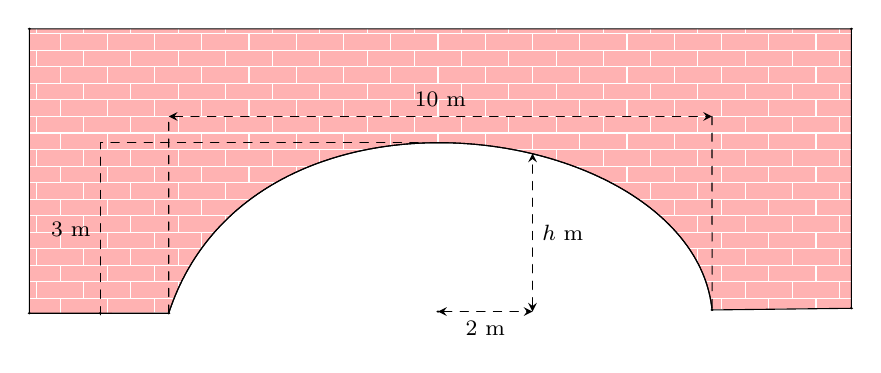
\begin{tikzpicture}[yscale=0.7,scale=.6,font=\footnotesize, line join=round, line cap=round, >=stealth]
			\coordinate (A) at (-8.65,-3.95);
			\coordinate (B) at (-8.65,4.65);
			\coordinate (C) at (8.75,4.65);
			\coordinate (D) at (8.75,-3.8);
			% Lát nền gạch
			\begin{scope}
				% Giới hạn vùng vẽ trong tứ giác ABCD
				\clip (A) -- (B) -- (C) -- (D) -- cycle;
				
				% Tham số viên gạch
				\def\brickwidth{1}
				\def\brickheight{0.5}
				
				% Vẽ từng viên gạch (nằm ngang, so le hàng)
				\foreach \y in {-4,-3.5,...,5} {
					\pgfmathsetmacro\offset{mod(\y/\brickheight,2)==0 ? 0 : \brickwidth/2}
					\foreach \x in {-10,-9,...,10} {
						\path[fill=red!30, draw=white]
						({\x*\brickwidth + \offset}, \y)
						rectangle ++(\brickwidth, \brickheight);
					}
				}
			\end{scope}
			\coordinate (E) at (-5.7,-3.95);
			\coordinate (F) at (5.8,-3.85);
			\coordinate (G) at (5.40,1.85);
			\coordinate (H) at (-3.9,3.9);
			\coordinate (I) at (-7.15,-3.95);
			\coordinate (J) at (-7.25,1.9);
			\coordinate (K) at (0,-3.9);
			\begin{scope}
				\draw[fill=white] (E) .. controls (H) and (G) .. (F);
			\end{scope}
			\draw (E) .. controls (H) and (G) .. (F);
			\fill (A) circle (1pt) (B) circle (1pt) (C) circle (1pt) (D) circle (1pt) (E) circle (1pt)(F) circle (1pt);
			\fill (I) circle (1pt)(K) circle (1pt);
			\draw (E)--(A)--(B)--(C)--(D)--(F) ;
			\draw[dashed] (E)--(-5.7,2) (5.8,2)--(F);
			\draw[dashed,<->](-5.7,2)--(5.8,2)node[midway,above]{$10$ m};
			\draw[dashed](-7.15,-4)--++(90:5.2)node[midway,left]{$3$ m} --++(0:6.9);
			\draw[dashed,<->](K)--++(0:2)node[midway,below]{$2$ m};
			\draw[dashed,<->](2,-3.9)--++(90:4.78)node[midway,right]{$h$ m};
		\end{tikzpicture}
	\end{center}
	\shortans{2,75 }
	\loigiai{
		Chọn hệ trục tọa độ $Oxy$ sao cho gốc $O$ trùng với tâm của đường hầm, trục $Ox$ nằm ngang theo chiều rộng của đường hầm, và trục $Oy$ thẳng đứng theo chiều cao của mái vòm.
		\begin{center}
			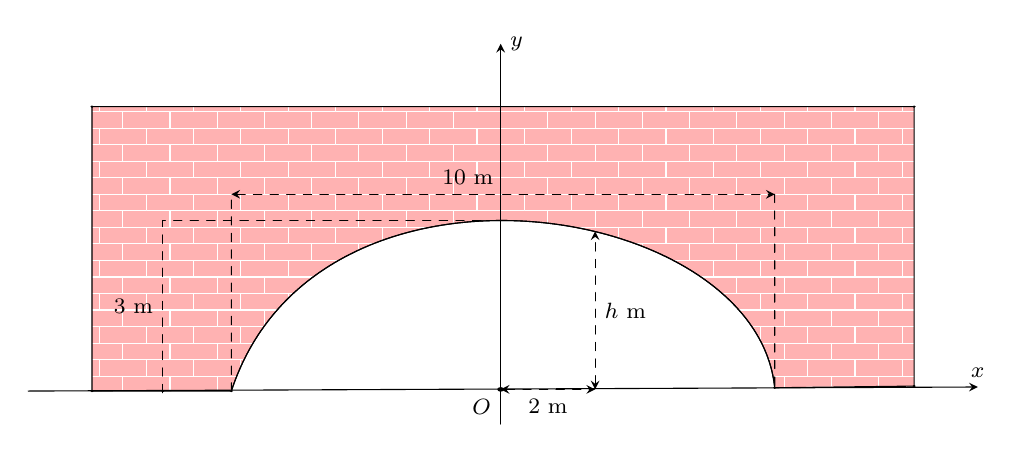
\begin{tikzpicture}[yscale=0.7,scale=.6,font=\footnotesize, line join=round, line cap=round, >=stealth]
				\coordinate (A) at (-8.65,-3.95);
				\coordinate (B) at (-8.65,4.65);
				\coordinate (C) at (8.75,4.65);
				\coordinate (D) at (8.75,-3.8);
				% Lát nền gạch
				\begin{scope}
					% Giới hạn vùng vẽ trong tứ giác ABCD
					\clip (A) -- (B) -- (C) -- (D) -- cycle;
					
					% Tham số viên gạch
					\def\brickwidth{1}
					\def\brickheight{0.5}
					
					% Vẽ từng viên gạch (nằm ngang, so le hàng)
					\foreach \y in {-4,-3.5,...,5} {
						\pgfmathsetmacro\offset{mod(\y/\brickheight,2)==0 ? 0 : \brickwidth/2}
						\foreach \x in {-10,-9,...,10} {
							\path[fill=red!30, draw=white]
							({\x*\brickwidth + \offset}, \y)
							rectangle ++(\brickwidth, \brickheight);
						}
					}
				\end{scope}
				\coordinate (E) at (-5.7,-3.95);
				\coordinate (F) at (5.8,-3.85);
				\coordinate (G) at (5.40,1.85);
				\coordinate (H) at (-3.9,3.9);
				\coordinate (I) at (-7.15,-3.95);
				\coordinate (J) at (-7.25,1.9);
				\coordinate (K) at (0,-3.9);
				\begin{scope}
					\draw[fill=white] (E) .. controls (H) and (G) .. (F);
				\end{scope}
				\draw (E) .. controls (H) and (G) .. (F);
				\fill (A) circle (1pt) (B) circle (1pt) (C) circle (1pt) (D) circle (1pt) (E) circle (1pt)(F) circle (1pt);
				\fill (I) circle (1pt)(K) circle (1pt);
				\draw (E)--(A)--(B)--(C)--(D)--(F) ;
				\draw[dashed] (E)--(-5.7,2) (5.8,2)--(F);
				\draw[dashed,<->](-5.7,2)--(5.8,2)node[midway,above left]{$10$ m};
				\draw[dashed](-7.15,-4)--++(90:5.2)node[midway,left]{$3$ m} --++(0:6.9);
				\draw[dashed,<->](K)--++(0:2)node[midway,below]{$2$ m};
				\draw[dashed,<->](2,-3.9)--++(90:4.78)node[midway,right]{$h$ m};
				\draw[->] (-10,-3.95)--++(.35:20.1) node[above] {$x$};
				\draw[->] (0,-4.95)--++(90:11.5) node[right] {$y$};
				\fill (0,-3.9) circle (2pt) node[below left] {$O$};
			\end{tikzpicture}
		\end{center}
		Phương trình của elip có dạng $\dfrac{x^2}{a^2} + \dfrac{y^2}{b^2} = 1$ $(a>b>0)$.\\
		Theo đề bài:\\
		Chiều rộng của đường hầm là $10$ m, đây là độ dài trục lớn $2a$. Vậy $2a = 10 \implies a = 5$ m.\\
		Điểm cao nhất của mái vòm là $3$ m, đây là độ dài nửa trục bé $b$. Vậy $b = 3$ m.\\
		Phương trình của nửa elip tạo thành mái vòm là $\dfrac{x^2}{5^2} + \dfrac{y^2}{3^2} = 1$ với $y \ge 0$.\\
		Hay $\dfrac{x^2}{25} + \dfrac{y^2}{9} = 1$.\\
		Ta cần tìm chiều cao $h$ (tức là giá trị của $y$) tại điểm cách tâm đường hầm $2$ m (tức là $x = 2$ m).\\
		Thay $x = 2$ vào phương trình elip
		$$\dfrac{2^2}{25} + \dfrac{h^2}{9} = 1 \Leftrightarrow h = \dfrac{3\sqrt{21}}{5}\approx 2{,}75\,\text{m}.$$
	}
\end{ex}
\Closesolutionfile{ans}

\begin{center}
	\textbf{PHẦN 4 - TỰ LUẬN}
\end{center}

\begin{ex}%[0H9V3-2]%[Dự án D - đợt 2 NH24-25- Quang Vinh NT]
	Trong mặt phẳng với hệ toạ độ $Oxy$, cho ba điểm $A(-1 ; 4)$, $B(1 ; 1)$, $C(4 ;-2)$.	
	\begin{enumerate}
		\item  Viết phương trình tổng quát của đường thẳng $A B$.
		\item  Trên đoạn thẳng $B C$, lấy điểm $M$ sao cho diện tích tam giác $A B M$ gấp đôi diện tích tam giác $ACM$. Viết phương trình đường thẳng $AM$.
	\end{enumerate}
	\loigiai{
		\begin{enumerate}
			\item   Đường thẳng $AB$  nhận véc-tơ $\overrightarrow{AB}=(2 ;-3)$ là một véc-tơ chỉ phương, nên nhận $\overrightarrow{n}=(3 ; 2)$ là một véc-tơ pháp tuyến.\\		 	
			Phương trình tổng quát của $AB\colon 	3(x-1)+2(y-1)=0 \Leftrightarrow 3 x+2 y-5=0	$.
			\item\hfill\\
			\begin{center}
				\begin{tikzpicture}[scale=1,line cap=round,line join=round,font=\footnotesize,>=stealth,declare function={c=0.65;kc=0.15;cao=6*c+3*kc;dai=1.65*cao;dait=dai/3;}]
					\path
					(0,0) coordinate (B)
					($(B)+(60:2)$) coordinate (A)
					($(B)+(0:4)$) coordinate (C)
					($(B)!(A)!(C)$)  coordinate (H)
					($(B)!2/3!(C)$) coordinate (M)
					;
					\draw (A)--(B)--(C)--(A)--(H) (A)--(M);
					\draw (H)--++(0:0.2)--++(90:0.2)--++(180:0.2);
					\foreach \p/\r in {A/90, B/180, C/-90,H/-90, M/-90}
					\fill (\p) circle (1.25pt) node[shift={(\r:3mm)}]{$\p$};
				\end{tikzpicture}	 
			\end{center}
			
			Gọi $AH$ là đường cao tam giác $ABC $. Ta có	
			\begin{eqnarray*}
				&& \mathrm{S}_{\triangle A B M}=\dfrac{A H \cdot B M}{2};\,  \mathrm{S}_{\triangle A C M}=\dfrac{A H \cdot C M}{2}\\
				&& \mathrm{S}_{\triangle A B M}=2 \mathrm{S}_{\triangle A C M}\Rightarrow B M=2 C M \\
				&& \Rightarrow \overrightarrow{B M}=2 \overrightarrow{M C} \Rightarrow \overrightarrow{O M}=\dfrac{1}{3}\left(2 \overrightarrow{O C}+\overrightarrow{OB}\right)=(3;-1)\\
				&& \Rightarrow M(3 ;-1).
			\end{eqnarray*}		 
			Đường thẳng $AM$ nhận véc-tơ $\overrightarrow{AM}=(4 ;-5)$ là véc-tơ chỉ phương, có phương trình $$\heva{&x=-1+4 t \\&y=4-5 t}\ (t\in \mathbb{R}).$$			 	
	\end{enumerate}	}
\end{ex}

\begin{ex}%[0H9H3-4]%[Dự án D - đợt 2 NH24-25- Quang Vinh NT]
	Trong mặt phẳng tọa độ $Oxy$, góc giữa hai đường thẳng $d_1\colon 2x + 3y - 1 = 0$ và $d_2\colon \heva{&x = 3 - 2t \\& y = 1 + 7t}$ bằng bao nhiêu độ (làm tròn kết quả đến hàng đơn vị)?
	\loigiai{
		Đường thẳng $d_2$ có véc-tơ chỉ phương là $\overrightarrow{u}_2 = (-2; 7)$. Suy ra véc-tơ pháp tuyến của $d_2$ là $\overrightarrow{n}_2 = (7; 2)$.\\
		Đường thẳng $d_1$ có véc-tơ pháp tuyến là $\overrightarrow{n}_1 = (2; 3)$.\\
		Ta có $\overrightarrow{n}_1 \cdot \overrightarrow{n}_2 = 2 \cdot 7 + 3 \cdot 2 = 20$; $|\overrightarrow{n}_1| = \sqrt{2^2 + 3^2} = \sqrt{13}$; $|\overrightarrow{n}_2| = \sqrt{7^2 + 2^2} = \sqrt{53}$.\\
		Gọi $\alpha$ là góc giữa đường thẳng $d_1$ và $d_2$.\\
		Khi đó $\cos \alpha = \dfrac{|\overrightarrow{n}_1 \cdot \overrightarrow{n}_2|}{|\overrightarrow{n}_1| \cdot |\overrightarrow{n}_2|} = \dfrac{20}{\sqrt{13} \cdot \sqrt{53}}$.\\
		Suy ra $\alpha \approx 40^\circ$.
	}
\end{ex}

\begin{ex}%[0H9V4-2]%[Dự án D - đợt 2 NH24-25- Quang Vinh NT]
	Trong mặt phẳng tọa độ $Oxy$, cho đường thẳng $d\colon x+y-3=0$ và điểm $M(-1;3)$.
	\begin{enumerate}
		\item Tính khoảng cách từ điểm $M$ đến đường thẳng $d$.
		\item Lập phương trình tổng quát của đường thẳng $\Delta$ biết $\Delta$ đi qua điểm $M$ và $N(-3;-1)$.
		\item Lập phương trình đường tròn $(C)$ biết tâm $I$ của đường tròn $(C)$ nằm trên đường thẳng $d$ và $(C)$ tiếp xúc với đường thẳng $\Delta$ tại điểm $M$.
	\end{enumerate}
	\loigiai{
		\begin{enumerate} \item Khoảng cách từ điểm $M(-1;3)$ đến đường thẳng $d\colon x+y-3=0$ là 
			\[\mathrm{d}(M,d) = \dfrac{|-1+3-3|}{\sqrt{1^2+1^2}} = \dfrac{|-1|}{\sqrt{2}} = \dfrac{1}{\sqrt{2}} = \dfrac{\sqrt{2}}{2}.\]
			\item Ta có $\overrightarrow{MN} = (-3 - (-1); -1 - 3) = (-2; -4)$. \\
			Đường thẳng $\Delta$ đi qua $M(-1;3)$ và có véc-tơ chỉ phương $\overrightarrow{u} = (-2;-4)$ nên có véc-tơ pháp tuyến $\overrightarrow{n} = (4;-2)$ hay $(2;-1)$. \\
			Phương trình tổng quát của đường thẳng $\Delta$ là \[2(x+1) - 1(y-3) = 0 \Leftrightarrow 2x+2-y+3=0 \Leftrightarrow 2x-y+5=0.\] 
			\item Gọi $I(x_I; y_I)$ là tâm đường tròn $(C)$. \\ Vì $I \in d$ nên $x_I+y_I-3=0 \Rightarrow y_I = 3-x_I$. \\ 
			Suy ra $I(x_I; 3-x_I)$. \\
			Gọi $d'$ là đường thẳng qua tâm $I$ và vuông góc với $\Delta$.\\
			Đường thẳng $d'$ đi qua $M(-1;3)$ và vuông góc với $\Delta\colon 2x-y+5=0$ có véc-tơ pháp tuyến là $\overrightarrow{n}_{d'} = (1;2)$. \\
			Phương trình đường thẳng $d'$ là 
			\[1(x+1)+2(y-3)=0 \Leftrightarrow x+2y-5=0.\]
			Vì $I \in d'$ nên 
			\[x_I+2(3-x_I)-5=0 \Leftrightarrow x_I=1.\] 
			Suy ra $y_I = 3-1=2$. \\ 
			Do đó $I(1;2)$. \\
			Bán kính đường tròn $(C)$ là 
			\[R = IM = \sqrt{(-1-1)^2+(3-2)^2} = \sqrt{5}.\] 
			Phương trình đường tròn $(C)$ là $(x-1)^2+(y-2)^2 = 5$.
		\end{enumerate}
	}
\end{ex}

